\section{Snímanie}

\begin{figure}[t]
    \centering
    \begin{subfigure}{0.3\textwidth}
        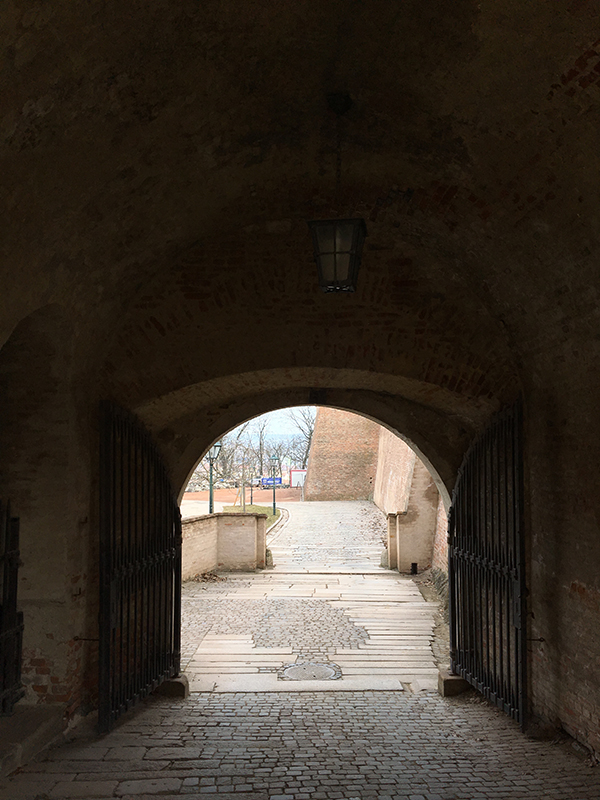
\includegraphics[width=\textwidth]{figures/capturing/exposures/underexposed}
        \caption{podexponovaná scéna}
        \label{fig:underexposed}
    \end{subfigure}
    ~
    \begin{subfigure}{0.3\textwidth}
        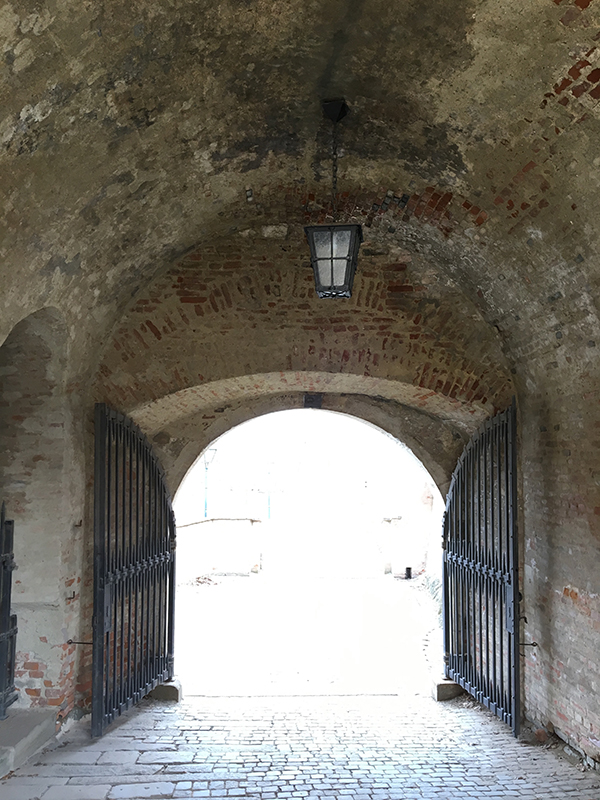
\includegraphics[width=\textwidth]{figures/capturing/exposures/overexposed}
        \caption{preexponovaná scéna}
        \label{fig:overexposed}
    \end{subfigure}
    \caption{Rozličné expozície rovnakej scény}
    \label{fig:exposed_scene}
\end{figure}

Je veľmi obtiažne zachytiť scénu (obr. \ref{fig:exposed_scene}), kde sú svetlé miesta mnohonásobne jasnejšie ako
tmavé miesta scény. To znamená, že takáto scéna má vysoký dynamický rozsah.
Rozličné nastavenia času expozície nám umožňujú vytvoriť fotografiu zachytávajúcu

a) veľmi svetlé (obr. \ref{fig:underexposed}) alebo

b) veľmi tmavé oblasti (obr. \ref{fig:overexposed}).

Na obrázku \ref{fig:pipeline} sú zobrazené technológie, ktorými je možné snímať, generovať
a zobrazovať scény s vysokým dynamickým rozsahom. Prvým problémom je zachytenie dynamického 
rozsahu scény. V súčasnosti existujú 3 metódy vytvárania HDR obsahu:
\begin{itemize}
    \item kombinovaním LDR snímok s rôznou hodnotou času expozície (obr. \ref{fig:pipeline} bod 1),
    \item zachytenie HDR scény špecializovaným hardvérom (obr. \ref{fig:pipeline} bod 2),
    \item virtuálne prostredia pomocou fyzikálne založených rendererov (obr. \ref{fig:pipeline} bod 3).
\end{itemize}

\begin{figure}[t]
    \centering
    \includegraphics[width=\textwidth]{figures/capturing/capturing_technologies}
    \caption{Dostupné technológie generovania HDR}
    \label{fig:pipeline}
\end{figure}

Kombinovanie viacerých snímok scény s rôznou hodnotou času expozície je pre svoju dostupnosť
a nenáročnosť najviac využívanou metódou. Dynamický rozsah reálneho sveta v rozpätí 
$10^{-3}$ $cd/m^{2}$ až $10^{6}$ $cd/m^{2}$ \cite{AHDR} je možné zachytiť na 8-bitov 
pre farebný kanál dekompozíciou tohoto rozsahu. Takto zachytíme detaily od najtmavšej,
až po najsvetlejšiu oblasť tak, ako je vyznačené na obrázku \ref{fig:expo_series}.

\begin{figure}[t]
    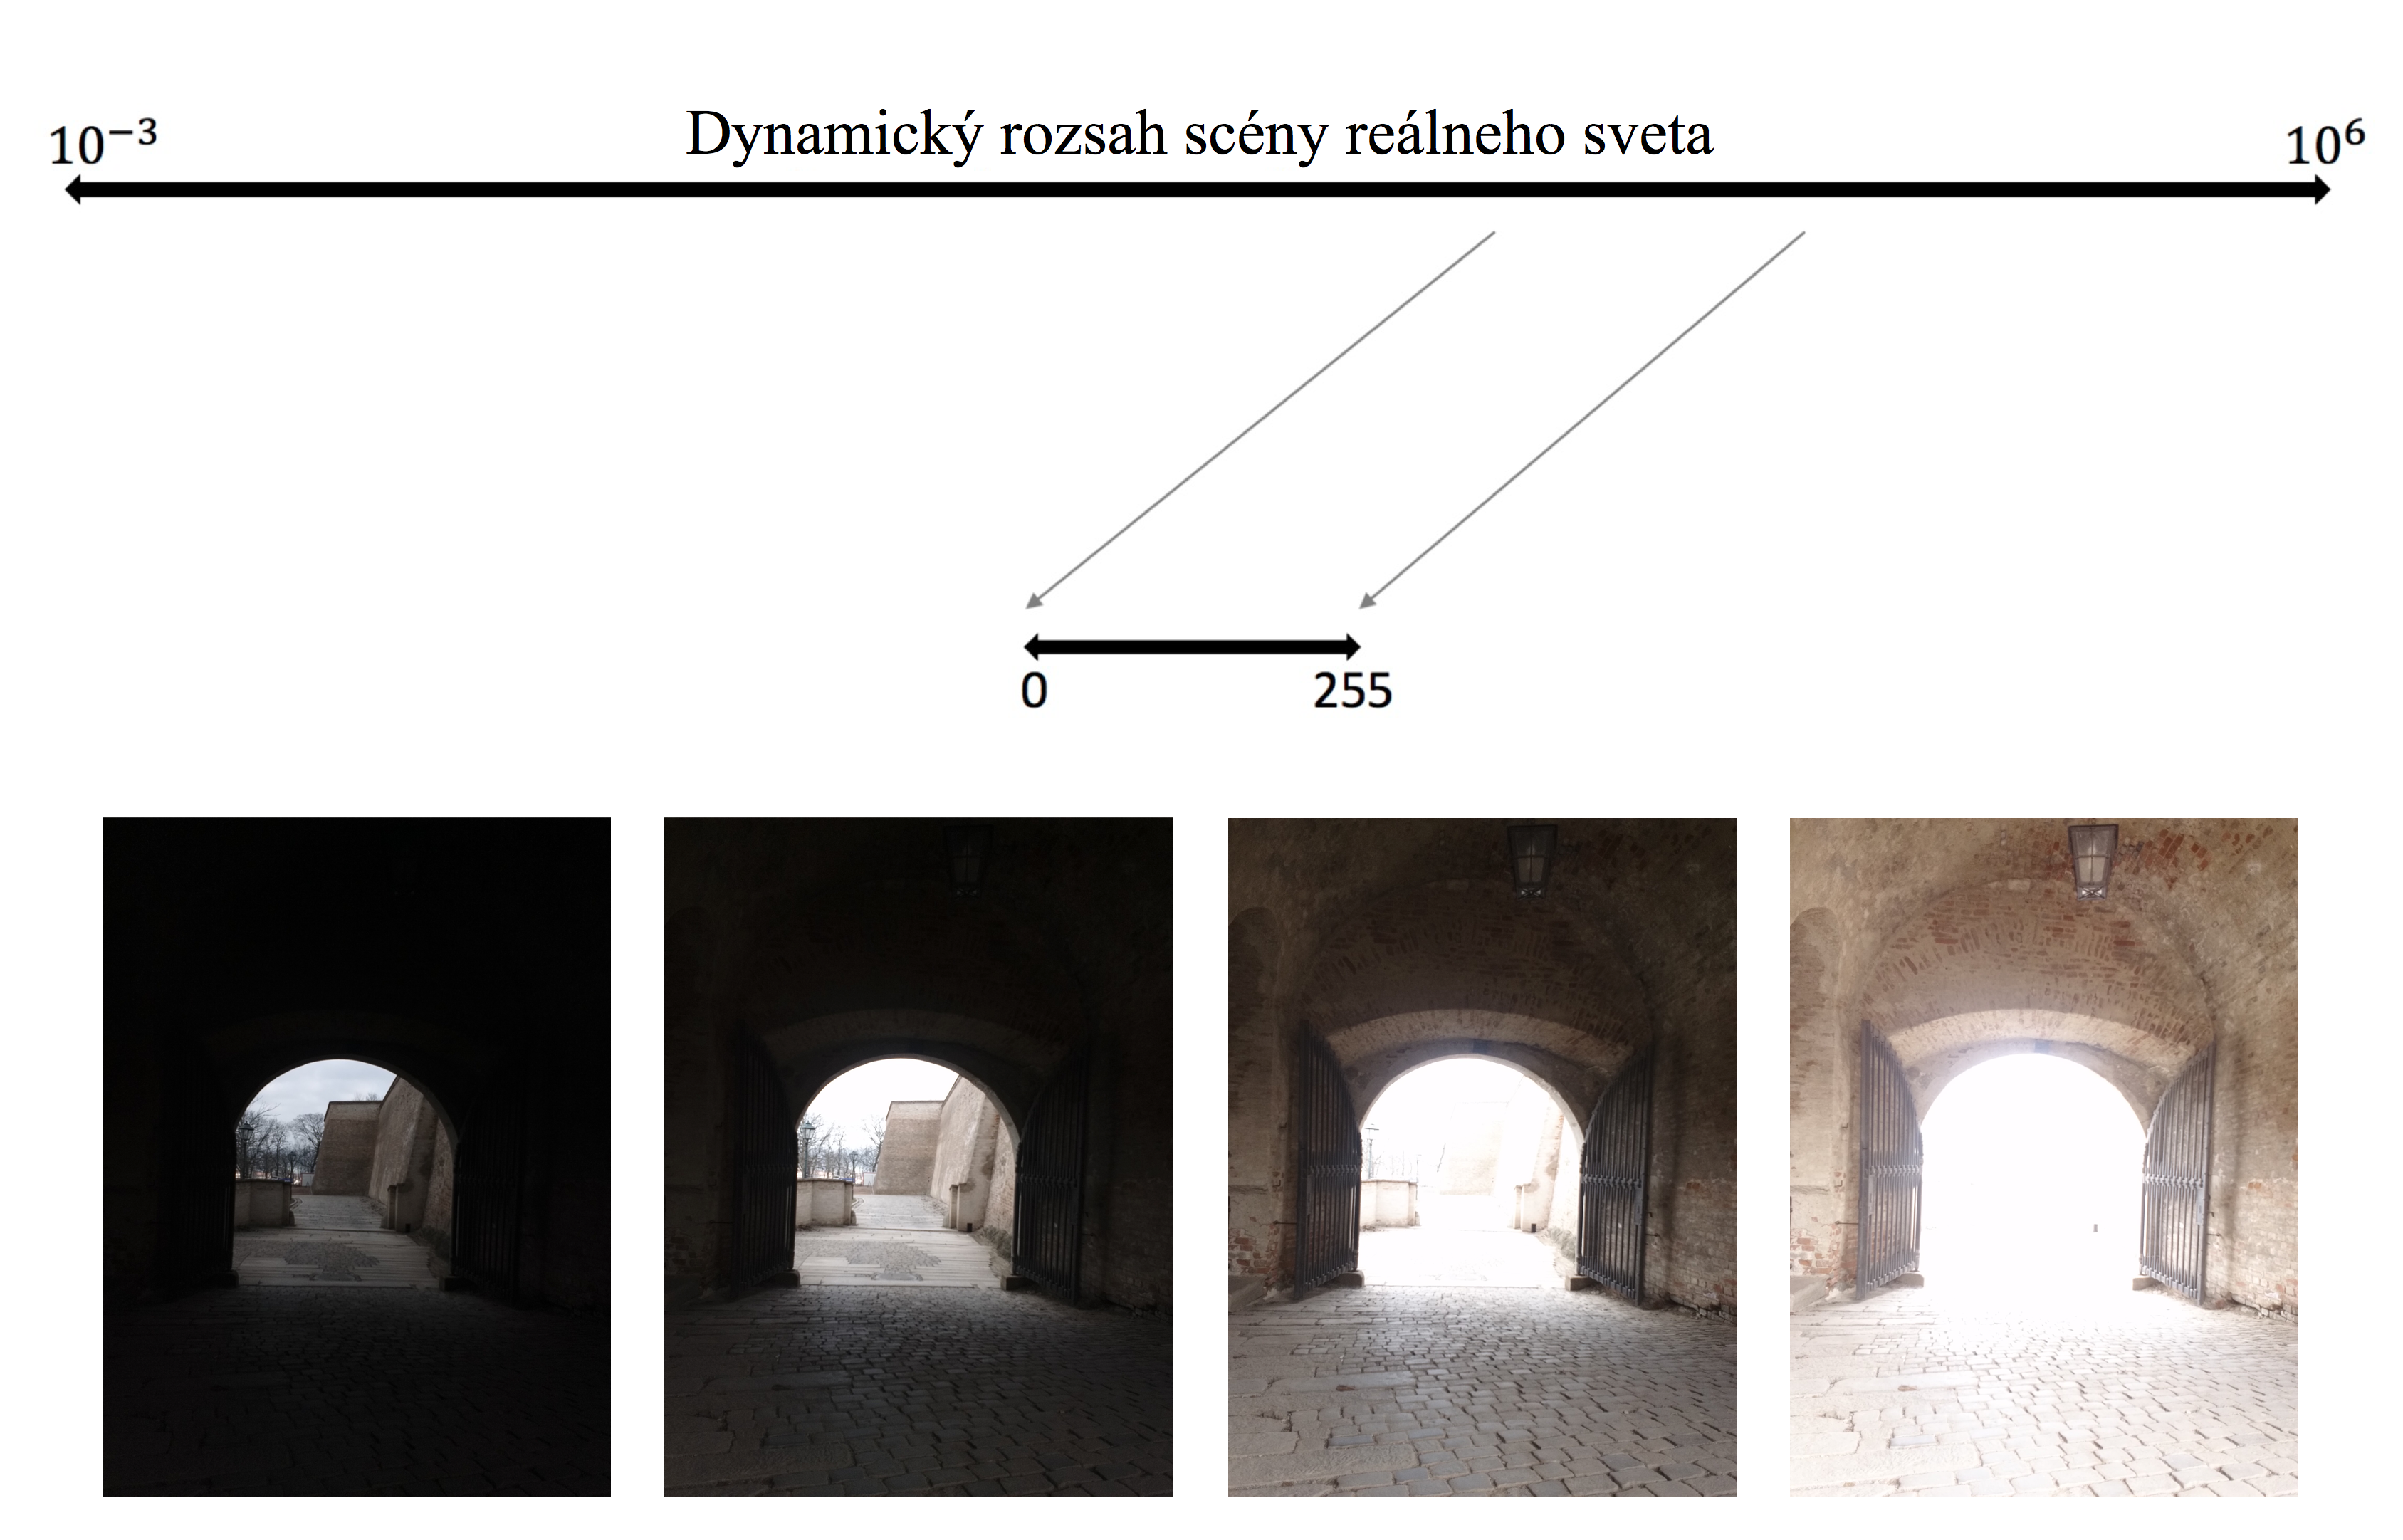
\includegraphics[width=\textwidth]{figures/capturing/capturing_series}
    \caption{Scéna zachytená snímkami s rôznymi hodnotami expozičného času}
    \label{fig:expo_series}
\end{figure}

\subsection{Parametre snímača}

Pred vytváraním fotografie s manuálnymi nastaveniami parametrov snímača je dobré poznať základné pojmy
\cite{ZakladyHDR}\cite{AHDR}:
\begin{description}
    \item [Expozícia] udáva celkové množstvo svetla dopadajúce na fotografické médium. Je závislá na čase expozície,
    clone a citlivosti ISO. Fotografia s nedostatočným množstvom svetla je podexponovaná a naopak fotografia s príliš
    veľkým množstvom svetla je preexponovaná.
    \item [Expozičný čas] udáva dobu, počas ktorej je svetlocitlivý snímač vystavený dopadajúcemu svetlu. Čím je hodnota
    expozičného času vyššia, tým viac svetla sa prepustí fo vnútra fotoaparátu a tým je snímka svetlejšia. Expozičný čas
    sa udáva v sekúndách, prípadne v zlomkoch sekundy (8, 4, 2, 1, 1/2, 1/4...).
    \item [Clona] vytvára otvor v objektíve, cez ktorý prechádza svetlo z vonkajšieho prostredia na~svetlocitlivý snímač
    fotoaparátu. Čím je clonové číslo nižšie, tým viac svetla sa prepúšťa do vnútra fotoaparátu. Clona ovplyvňuje
    expozíciu, hĺbku ostrosti a kresbu objektívu.
    \item [Citlivosť ISO] určuje mieru citlivosti snímača na dopadajúce svetlo. S rastúcou citlivosťou rastie miera šumu,
    ktorý sa prejavuje ako náhodne farebné pixely vo fotografii. Šum je zretelnejší hlavne v tmavých oblastiach a prejavuje
    sa tiež pri dlhších expozíciách vplyvom zahrievania snímača.
    \item [Hodnota expozície] (EV) je číslo, ktoré predstavuje kombináciu expozičného času a clonového čísla. Táto hodnota udáva
    určité množstvo zachyteného svetla zo scény pri pevne danej hodnote citlivosti ISO (obvykle ISO100). Pri kombinácii času
    expozície $t$ a clonového čísla $N$ je EV definované ako:
    $EV = \ln_{2}\frac{N^{2}}{t}$.
    \item [Snímač] fotoaparátu, alebo snímací čip, je umiestnený za objektívom a tvorí najdôležitejší prvok fotoaparátu.
    Dôležitými vlastnosťami snímačov fotoaparátu sú jeho rozmer (čím väčší rozmer, tým kvalitnejší výsledný obraz) a počet
    pixelov, z ktorých sa snímač skladá.

    Snímače sa podľa technológie výroby delia na CCD\footnote{Charge–Coupled Device} a CMOS\footnote{Complementary Metal Oxide Semiconductor}.
    Oba typy snímačov obsahujú maticu pixelov (senzorov), ktoré sú zložené zo subpixelov, vo väčšine prípadov usporiadaných do tzv.
    Bayerovej masky. Každý subpixel má priradený farebný filter, ktorý sa používa na filtrovanie dopadajúceho svetla a tým môže zaznamenať
    iba jednu farebnú zložku. Ak však na tento subpixel dopadne fotón, ktorého vlnová dĺžka reprezentuje inú farbu, akú je filter
    schopný prepustiť, stráca sa farebná informácia. CMOS čipy sú najpoužívanejším typom senzorov. Ich výroba je konštrukčne náročnejšia,
    ale majú nižšiu spotrebu energie a rýchlejší prenos dát. Dáta prenášajú z~každého bodu samostatne, zatiaľ čo CCD po celých riadkoch.
\end{description}

\subsection*{Rozdiel medzi LDR a HDR snímkami}

Hlavný rozdiel medzi LDR\footnote{low dynamic range} snímkami a snímkami HDR je v hodnotách pixelov.
Hodnoty pixelov v HDR sú vo všeobecnosti spájané s jasom. Pixely nevyjadrujú presné hodnoty
jasu, pretože fotoaparát má inú spektrálnu citlivosť ako ľudské oko, ale iba aproximujú 
fotometrické veličiny. Približná odchýlka od fotometrických meraní je v rozsahu od 10\% 
pre achromatické (šedé) povrchy až po 30\% pre farebné objekty \cite{DCmerania}.
